\documentclass[border=5mm]{standalone}
\usepackage{xcolor}
\definecolor{winered}{rgb}{0.8,0,0}
\usepackage{pgfplots,tikz}
\usetikzlibrary{arrows.meta}
\usepgfplotslibrary{
	colorbrewer,
}
\pgfplotsset{
	compat=1.13,
}
\usepackage[outline]{contour}
\contourlength{0.5pt}

\begin{document}
	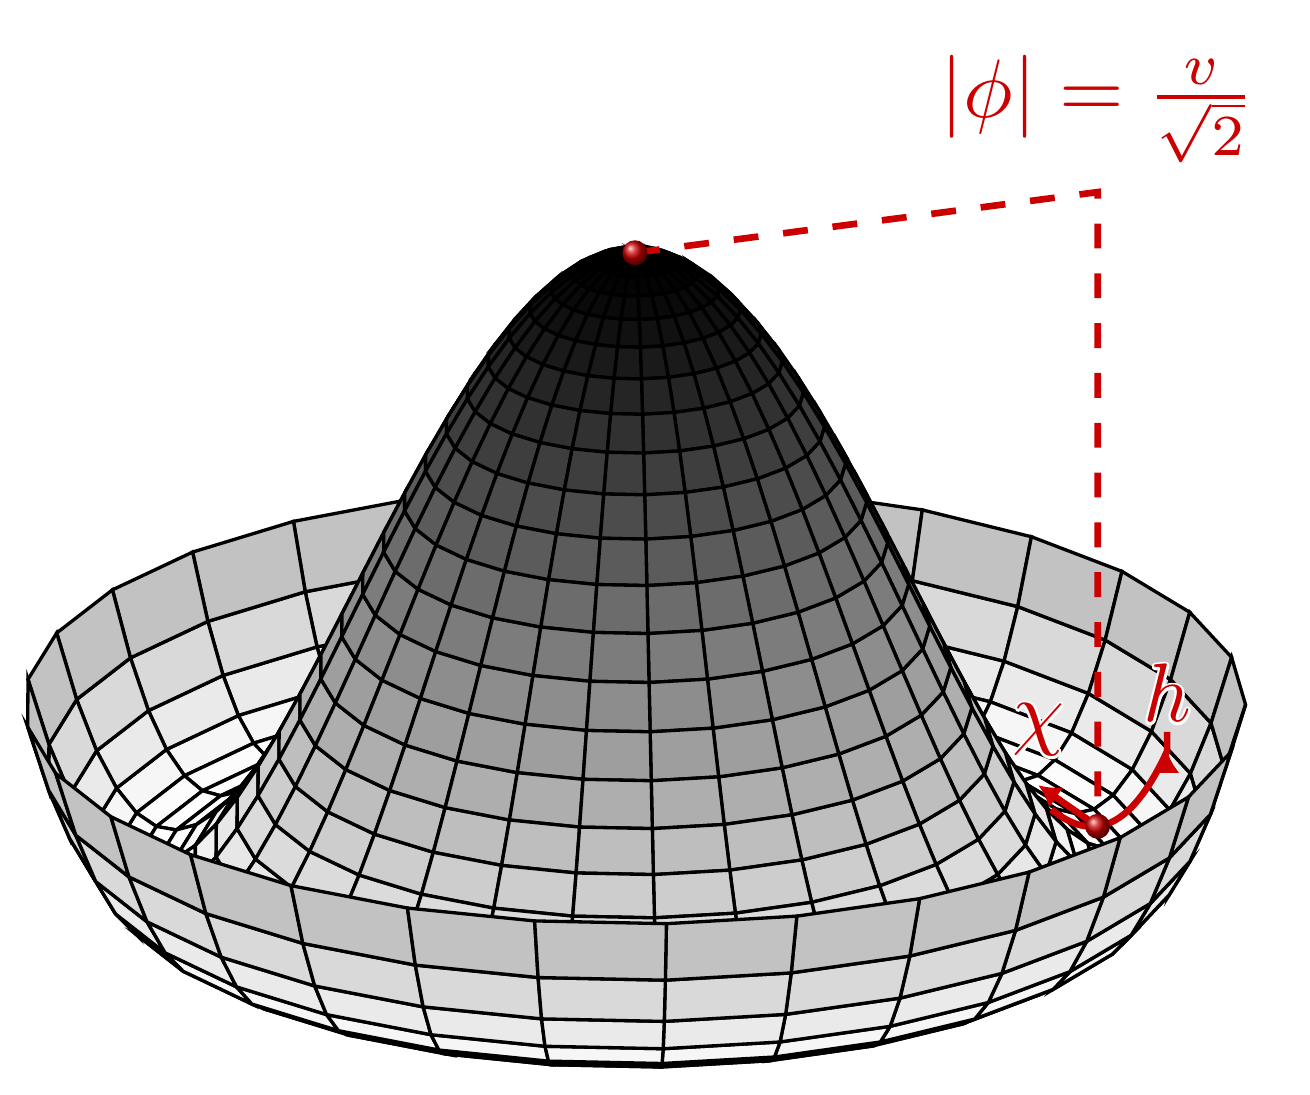
\begin{tikzpicture}[
		scale=3,
		smallarrowhead/.style={->,>={Latex[winered,angle=60:3pt]}},
		blob/.style={ball color=winered,shape=circle,minimum size=3pt,inner sep=0pt},
		]
		\pgfmathsetmacro{\vev}{0.246}
		\begin{axis}[
			% for debugging purposes only
			% view={0}{90},
			hide axis,
			data cs=polar,
			samples=30,
			domain=0:360,
			y domain=0:.305,
			declare function={
				higgspotential(\r)={(\r^2-\vev^2)^2};
				% functions to calculate cartesian coordinates from polar coordinates
				pol2cartX(\angle,\radius) = \radius * cos(\angle);
				pol2cartY(\angle,\radius) = \radius * sin(\angle);
			},
			colormap = {whiteblack}{color(0cm)  = (white);color(1cm) = (black)}
			]
			\pgfmathsetmacro{\angle}{45}
			\addplot3 [surf,shader=flat,draw=black,z buffer=sort] {higgspotential(y)};
			\addplot3 [winered,thick,smallarrowhead] coordinates {
				(\angle,\vev,{higgspotential(\vev)}) ({\angle+15},\vev,{higgspotential(\vev)})
			};
			\addplot3 [winered,thick,y domain={0.9*\vev}:{1.15*\vev},smallarrowhead] (\angle,y,{higgspotential(y)});
			\draw [winered,thick,dashed] (0,0,{higgspotential(0)})
			coordinate [style=blob]
			-- ({pol2cartX(\angle,\vev)},{pol2cartY(\angle,\vev)},{higgspotential(0)}) 
			-- ({pol2cartX(\angle,\vev)},{pol2cartY(\angle,\vev)},{higgspotential(\vev)})
			coordinate [style=blob];
			\node[anchor=south] at ({pol2cartX(\angle,\vev)},{pol2cartY(\angle,\vev)},{higgspotential(0)})                   {\color{winered}$\left\vert\phi\right\vert=\frac{v}{\sqrt{2}}$};
			\node[anchor=south] at ({pol2cartX(\angle+15,\vev)},{pol2cartY(\angle+15,\vev)},{higgspotential(\vev)})          {\contour{white}{\color{winered}$\chi$}};
			\node[anchor=south] at ({pol2cartX(\angle,1.15*\vev)},{pol2cartY(\angle,1.15*\vev)},{higgspotential(1.15*\vev)}) {\contour{white}{\color{winered}$h$}};
		\end{axis}
	\end{tikzpicture}
	
\end{document}